
\documentclass[11pt]{article}

\usepackage{common}
\usepackage{amsmath}
\usepackage{hyperref}
\usepackage{graphicx}

\title{HW2: Tagging from Scratch}
\author{Virgile Audi \\ Kaggle ID: Virgile Audi \\ vaudi@g.harvard.edu \and Nicolas Drizard \\ Kaggle ID: nicodri \\ nicolasdrizard@g.harvard.edu }
\begin{document}

\maketitle{}
\section{Introduction}

This assignement aims to tackle the task of part-of-speech tagging based on the paper by \cite{Collobert}.

We applied several models, both in terms of the features used and of the models. First, we applied a multi-class Naive Bayes and then a Multinomial Logistic Regression. We used slicing window features with information from the words and capitalization. We tried both with and without the position of the words inside the window.

Then, we used a neural network architecture with two layers. We ran several experiments on this model which was the most accurate. For instance, we trained it on a pre-trained embeddings of words from \cite{pennington}. This lead to our best prediction on the test set.

$$\text{http://github.com/virgodi/cs287}$$

This repository also contains iTorch notebooks where we drafted code.


\section{Problem Description}

The problem to solve is mult-class classification of tags on words, aka part-of-speech tagging based.\\


We have a training set of around 600 000 words in sentences, and a validation and test set of both around 100 000 words. We pre-processed them to extract in slicing windows of 5 words a vector of word-index and a vector of capitalisation feature for each word. We followed the conventions used by \cite{Collobert}. The words-index were extracted from the dictionary of words of the embeddings. For the capitalisations features, we used the following values:
\begin{itemize}
\item 1: lower case words
\item 2: capital letter feature
\item 3: first letter in caps
\item 4: else
\end{itemize}

The output is a set of 45 classes of tags. We evaluated our model on the validation set to tune the hyperparameters.


\section{Model and Algorithms}

We present here in more details each model with its specificity and the different algorithms we used.

\subsection{Multinomial Naive Bayes}

The multinomial Naive Bayes \cite{murphy2012machine} is a generative model, it means that we specify the class conditional distribution $p(\boldx | y=c)$ as a multinoulli distribution. The main assumption here, which  justifies the 'naive' name, is that the feature are condionnaly independent given the class label.\\ \\
The goal is then to select the parameters that maximizes the likelihood of the training data:
    \[p(\boldy = \boldmath{\delta(c)}) = \sum_{i = 1}^n \frac{1(\boldy_i = c)}{n}\]

\noindent With the chain rule and the independency assumption we canc ompute the likelihood as follows:

\[ p(\boldy = c | x) \propto p(\boldy = c) \prod_{f \in \mathcal{F}} p(x_f| \boldy=\boldmath{\delta(c)})\]

\noindent We compute $p(x_f| \boldy=\boldmath{\delta(c)})$ with a count matrix. In our case, we have both the features related to the words and the caps, as they are independent we can treat each relative window position as a separate multinomial distribution which will give:

\[ p(x| \boldy=\boldmath{\delta(c)}) = \prod_{i = -d_{win}/2}^{i =d_{win}/2} p(\text{word at i in x}| \boldy=\boldmath{\delta(c)}) p(\text{capitalisation at i in x} | \boldy=\boldmath{\delta(c)}))\]


\noindent We use the count matrix $\boldF$ of both the words features and the capitalization one. The global definition is the following one:
\[F_{f,c} = \sum_{i = 1}^n \mathbf{1}(\boldy_i = c) \mathbf{1}(x_{i, f} = 1) \mathrm{\ for all\ } c\in \mcC, f\in \mcF\] 
Then,
      \[p(x_f = 1 | \boldy=\boldmath{\delta(c)}) = \frac{F_{f, c}}{\displaystyle \sum_{f' \in \mcF} F_{f',c}}  \]

\noindent We can add a hyperparameter to handle the long tail of words by distributing the means. We add a Laplacian smoothing parameter $\alpha$ as follows:

  \[\hat{\boldF} = \alpha + F\]

\subsection{Multinomial Logistic Regression}

As a second baseline model, we implement a multiclass logistic regression for this problem. We won't recall the theoretical framework from homework 1 here, but will explain how it applies to speech tagging.\\

\noindent For this particular problem of speach tagging, we had the two same set of input features as for the Naive Bayes approach, i.e. the word windows as well as the capital windows. The main difference however is that for fitting this particular model, we needed to create some new features based on the position of the word and the type of capitalisation in the window. To do so we indexed words in first position from 1 to 100 002 (the size of the vocabulary), words in second position from 100 003 to 200 004, etc. For instance if the first training point was originally represented by: 
$$ \left(1 \quad 1 \quad 5032 \quad 2 \quad 4\right),$$ \noindent it was now inputed as:

$$ \left(1 \quad 100\, 003 \quad 205\, 036 \quad 300\, 008 \quad 400\, 014\right)$$

\noindent In total, we needed to fit 100 002x5 = 500 010 parameters. After writing a functional explicit stochastic gradient descent algorithm, we decided to use the more optimised function \newline \textbf{nn.StochasticGradient()} in order to gain some valuable training time. This function, for which documentation can be found on \href{https://github.com/torch/nn/blob/master/doc/training.md}{here} (hyperlink), takes for input a dataset with a special table structure, the model itself and the criterion. We can also tune the learning rate and number of epochs to run. It is not clear though what the size of the minibatch is but the function was fast enough not to worry about it.\\

\noindent As the primary goal of this homework was building the neural network, we did not intensively work on the Logistic Regression and kept it rather simple, only implementing a version that only took into consideration the word windows. We will present the results in the Experiments section.
 
\subsection{Neural Network Model}

We then focused on the primary objective of the homework which was building a neural network for word tagging. The model is designed as follows. \\

\noindent We input both word and cap windows, both of dimension 5. Each of these windows are then passed through look-up tables of dimensions dim(Vocabulary) x (hidden-parameter) and dim(Cap) x (hidden-parameter) . For each window, this outputs a 5xhidden-parameter tensor. We then concatenate corresponding tensors for a particular window to form a vector of dimension 1x(10$*$hidden-parameter).\\

\noindent We then applied a linear transformation to this vector followed by a layer to extract highly non-linear features in the form of a hardtanh() module. The output of this hardtanh() module is then passed through an other linear layer  to output a score for each of the 45 possible tags, followed by a softmax() module to transform these scores into a probability distribution over these tags. \\

\noindent This design therefore introduces to hidden parameters that need to be tuned, the dimension of the look-up table and the dimension of the output of the first Linear layer. We will present various experiments below.\\

\noindent In order to simplify the code and be able to use the nn.StochasticGradient() function to train the neural network and taking into account that it only takes a single datastructure argument, we chose to reformat the input data. Instead of having to deal with two different input tensors, i.e. the word and caps tensors, we concatenated the into one single tensor of size: dim(train) x 10. To be able to then use a single Look-up table, we had to index the caps from 100 003 to 100 006 and count them as extra words.

\noindent We would now like to share a trick that helped us run the code. When first coded the Sequential module in Torch, we had issues passing from the concatenation step to the first linear layer due to dimension issues in minibatching. Debugging the code, we noticed that the outputed tensor from the concatenation had an extra unnecessary 1 dimension that came from applying the nn.View() layer. As suggested in the following \href{https://groups.google.com/forum/#!topic/torch7/u4OEc0GB74k}{discussion tread} , we implemented a nn.Squeeze() layer similar to the nn.View() in order to transfer what the torch.Squeeze() function did to remove unwanted 1D dimensions in a tensor.\\

\noindent The url of the group is: https://groups.google.com/forum/\#!topic/torch7/u4OEc0GB74k\\

\noindent We now present results of the experiments.

\section{Experiments}

\subsection{Naive Bayes}

We first tried the Naive Bayes on the windowed features without considering the index of the words inside the window. The results were pretty bad (even if we tuned the hyperparameter):
\begin{itemize}
	\item Training Accuracy: \textbf{37 \%}
	\item Test Accuracy: \textbf{35 \%}
\end{itemize}

As a result, we decided to use the features described in the multinomial logistic regression part. This provided better results. We were able then to tune the alpha parameter with the accuracy value on the validation set.

\begin{figure}[H]
\centering
\begin{minipage}{.4\textwidth}
  \centering
  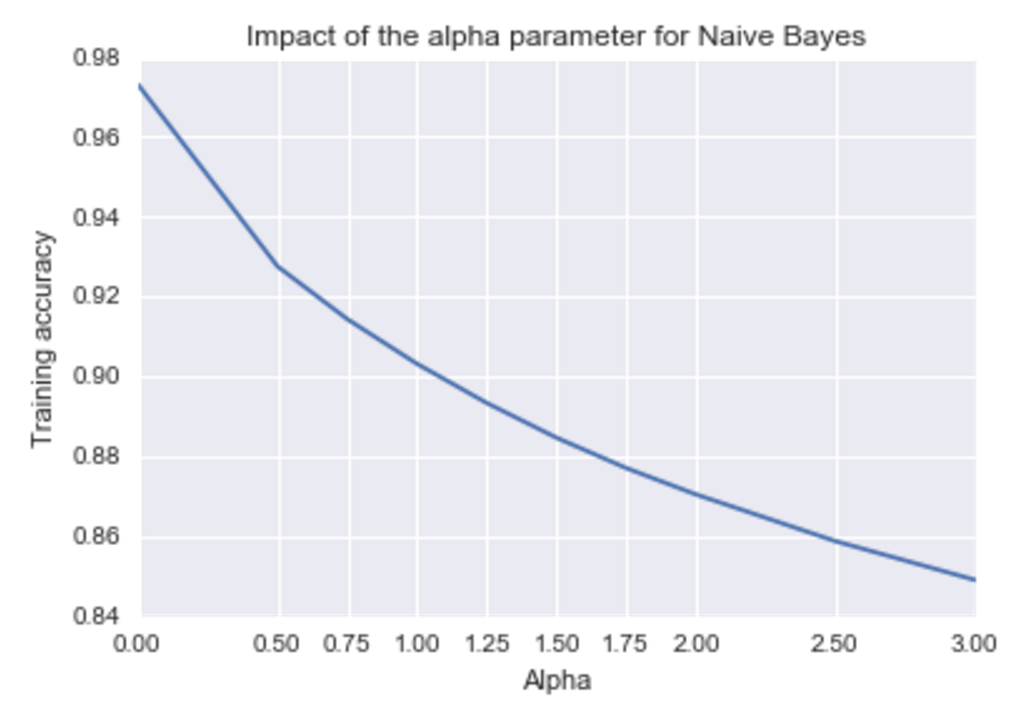
\includegraphics[width=1.2\linewidth]{training_nb}
\end{minipage} 
\hfill
\begin{minipage}{.4\textwidth}
  \centering
  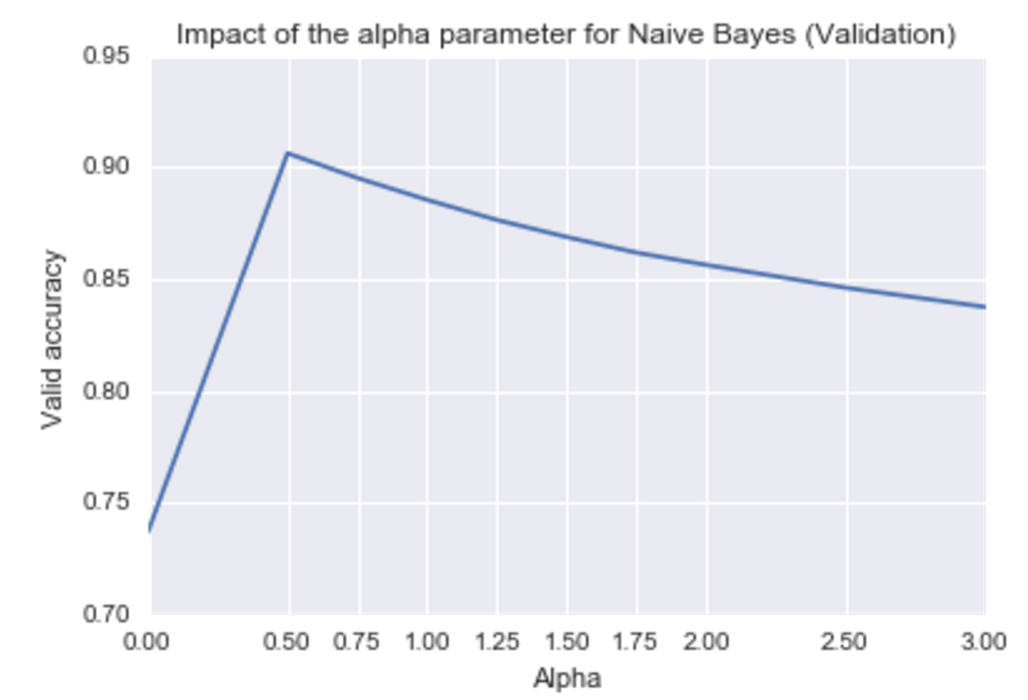
\includegraphics[width=1.2\linewidth]{validation_nb}
\end{minipage}
\end{figure}

The plots demonstrate how the Naive Bayes is prone to overfitting and also the impact of the alpha parameter. In deed we see that the accuracy keeps decreasing on the training set when alphas increase but on the validation set it has a maximum on $\alpha = 0.5$. The accuracy reached are still lower than those reached with the neural network architecture but it provides a good result with regards to the really low training time: \textbf{30 seconds}


\subsection{Linear Regression}
As mentioned earlier, we did not run exhaustive tests as it was more of a warm-up. We present the results of a test made with a learning rate of 0.01:

\begin{figure}[h]
\centering
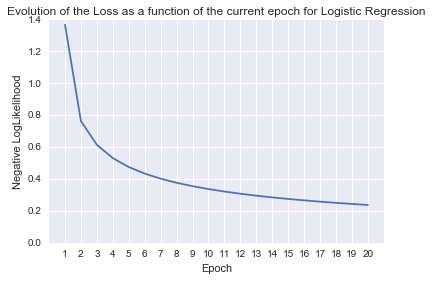
\includegraphics[width=9.5cm]{logReg_err}
\end{figure}

\noindent This lead to the following accuracy results:

\begin{table}[H]
\centering
\label{my-label}
\begin{tabular}{|c|c|c|}
\hline
Training & Validation & Test    \\ \hline
92.99\%  & 91.04\%    & 91.93\% \\ \hline
\end{tabular}
\caption{Accuracy for Multiclass Logistic Regression}
\end{table}

\noindent Based on the shape of the Loss curve, we thought running the algorithm for some extra epochs would not improve the accuracy drastically and decided to focus on the next part of the problem, the neural network.

\subsection{Neural Network}

We started by running the simplest model by setting the 2 hidden parameters to be equal to 50. As for the Linear regression model, we plot the loss function:

\begin{figure}[H]
\centering
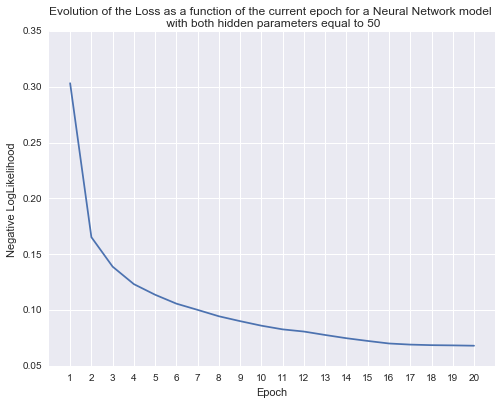
\includegraphics[width=9.5cm]{nn1}
\end{figure}

\noindent As one can observe, the starting loss for the neural network is almost equal to final loss obtained for the LogReg model ! We also note that we observe the same phenomenum of platauing. After 5-6 epochs, the improvements in the loss are incremental. Regarding accuracy, we submitted an entry for this particular model for the Kaggle Competetion and obtained the following results:

\begin{table}[H]
\centering
\label{my-label2}
\begin{tabular}{|c|c|c|}
\hline
Training & Validation & Test    \\ \hline
97.48\%  & 95.92\%    & 93.47\% \\ \hline
\end{tabular}
\caption{Accuracy for Neural Network}
\end{table}

\noindent We trained some other models with different parametrisation but did not notice major improvements in term of accuracy and loss. So we decided to pursue by adding the pre-embeddings for the words. Using these values as starting points for the words parameter helped us enormously as it constrained the first hidden parameter to 50 and allowing us to concentrate more computational ressources on tuning the second hidden parameter corresponding to the second linear layer.\\

\noindent We used 6 values for training: $$40, \quad 50, \quad 60, \quad 80, \quad 100, \quad 120$$

\noindent We present various plots to illustrate the results. We first show the evolution of the loss function, and we add both previous losses in order to compare:

\newpage
\begin{figure}[H]
\centering
\begin{minipage}{.4\textwidth}
  \centering
  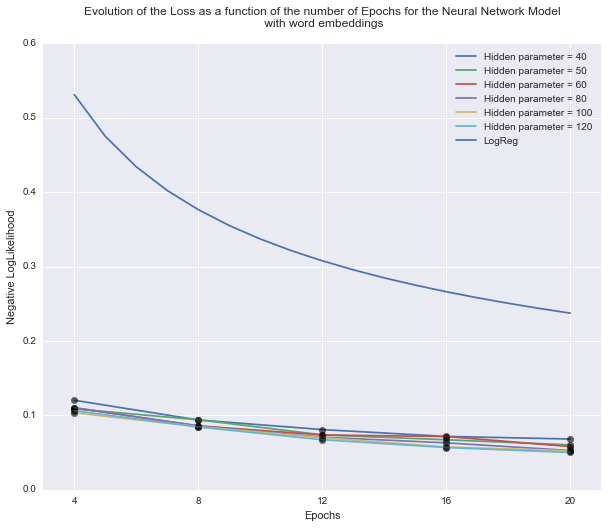
\includegraphics[width=1.2\linewidth]{compa}
\end{minipage} 
\hfill
\begin{minipage}{.4\textwidth}
  \centering
  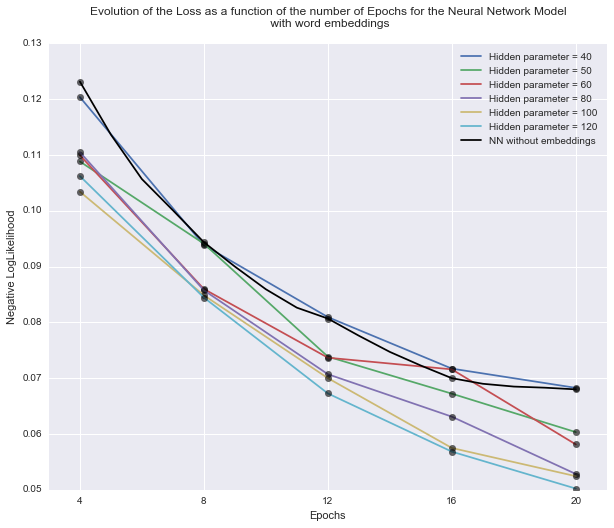
\includegraphics[width=1.2\linewidth]{nn_embed}
\end{minipage}
\end{figure}

\noindent This shows how much adding the embeddings helped reach better results in terms of loss but also in terms of accuracy on both train and validation:

\begin{figure}[H]
\centering
\begin{minipage}{.4\textwidth}
  \centering
  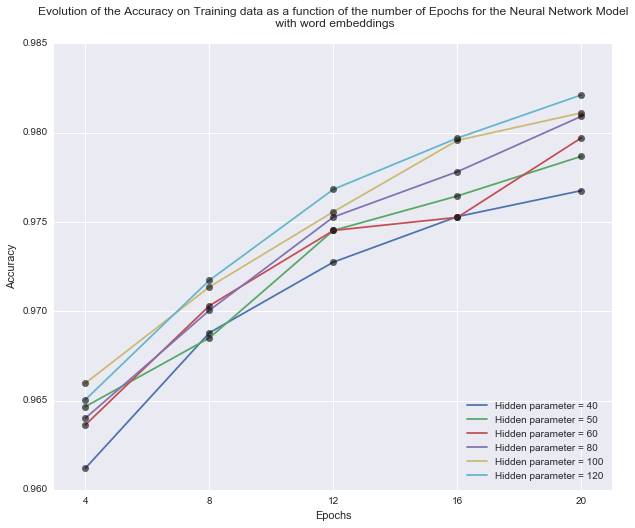
\includegraphics[width=1.2\linewidth]{train_nn}
\end{minipage} 
\hfill
\begin{minipage}{.4\textwidth}
  \centering
  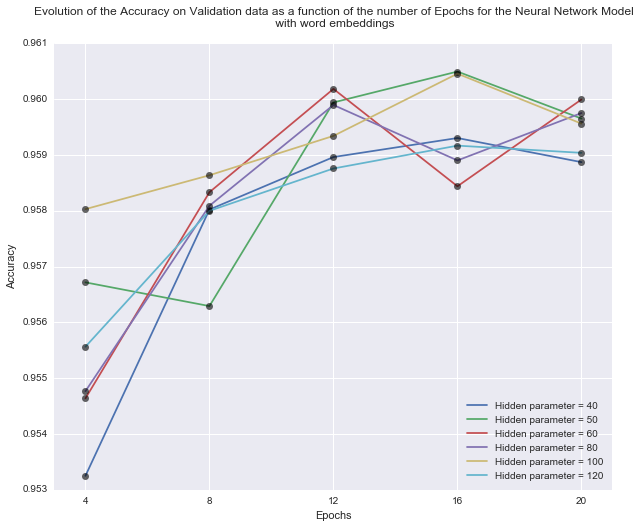
\includegraphics[width=1.2\linewidth]{valid_nn}
\end{minipage}
\end{figure}

We decided to submit the predictions of the models with highest validation accuracy since the performance on the training sets were very close and we also wanted to avoid overfitting. We obtained:

\begin{table}[H]
\centering
\label{my-label2}
\begin{tabular}{|c|c|c|}
\hline
Training & Validation & Test    \\ \hline
97.97\%  & 95.99\%    & 96.19\% \\ \hline
\end{tabular}
\caption{Accuracy for Neural Network with word embeddings and HP2 = 60}
\end{table}

\noindent If we look at training times (that also include evaluating intermediate accuracies), we can see that they seem pretty reasonable for 20 epochs:\\

\begin{table}[H]
\centering
\label{my-label3}
\begin{tabular}{|c|c|c|c|c|c|c|}
\hline
HP2      & 40   & 50   & 60   & 80   & 100  & 120  \\ \hline
Time (s) & 5532 & 5636 & 5730 & 5916 & 6100 & 7126 \\ \hline
\end{tabular}
\caption{Run Times}
\end{table}

\noindent We topped the Kaggle competition for some time but eventually lost our lead. To try to regain it, we tried some new experiments. We first tried to fix the embeddings at each epoch but obtained strange results probably due to a coding issues (more info can be found in the notebooks). We also tried to add an extra Hardtanh layer followed by another linear one. Results were not as good as expected and we decided to not pursue this lead any further. We show results for 2 differents parametrisations: 50,50,50 and 50,70,50. We used the embeddings that forced us to use 50 as our first hidden parameter.

\begin{table}[H]
\centering

\label{my-label}
\begin{tabular}{|c|c|c|c|}
\hline
Accuracy on & \multicolumn{1}{c|}{Train} & \multicolumn{1}{c|}{Valid} & Test    \\ \hline
50, 50, 50  & 96,73\%                    & 95.62\%                    & XXX     \\ \hline
50, 70, 50  & 96.89\%                    & 95.90\%                    & 95.98\% \\ \hline
\end{tabular}
\caption{Accuracy for Neural Network with Extra Layer}
\end{table}


\section{Conclusion}

As we can see, a rather simple neural network clearly outperforms both Naive Bayes and Logistic Regression for word tagging. If there is no possibilities to beat Naive Bayes in terms of run time, the Neural Network is as fast or even faster to train than Logistic Regression as in order to work for word tagging, the number of parameters to infer is much more important in the latter. We unfortunately did not succeed in improving the results by changing the architecture of the network but observed some major improvements by addind the word embeddings from \cite{pennington}.



\bibliographystyle{apalike}
\bibliography{HW1.bib}

\end{document}
